\documentclass[svgnames,11pt]{beamer}
\input{/home/tof/Documents/Cozy/latex-include/preambule_commun.tex}
\input{/home/tof/Documents/Cozy/latex-include/preambule_beamer.tex}
\usepackage{pgfpages} \setbeameroption{show notes on second screen=left}
\author[]{Christophe Viroulaud}
\title{Principe du routage}
\date{\framebox{\textbf{Archi 10}}}
%\logo{}
\institute{Terminale - NSI}

\begin{document}
\begin{frame}
    \titlepage
\end{frame}

\begin{frame}
    \frametitle{}


    \begin{center}
        Juin 2020: 1,78 milliards de sites web
    \end{center}
    \begin{framed}
        \centering Comment retrouver une machine dans un réseau?
    \end{framed}
    \note{Le réseau internet permet de communiquer avec n’importe quelle machine connectée.}
\end{frame}
\section{Protocoles de communication}
\begin{frame}
    \frametitle{Protocoles de communication}


    \begin{aretenir}[]
        \textbf{Protocole:} ensemble de règles qui définissent comment se produit une communication dans un réseau.
    \end{aretenir}

\end{frame}
\begin{frame}
    \frametitle{}

    \begin{center}
        \renewcommand{\arraystretch}{1.5}
        \begin{tabular}{|c|}
            \hline
            \textbf{Application}                  \\
            \hline
            \textbf{Transport} ou \textbf{TCP}    \\
            \hline
            \textbf{Internet} ou \textbf{IP}      \\
            \hline
            \textbf{Réseau} ou \textbf{Interface} \\
            \hline
        \end{tabular}
        \renewcommand{\arraystretch}{1}
        \captionof{table}{Protocole TCP/IP (1970)}
    \end{center}
    \note{TCP: Transmission Control Protocol}
\end{frame}
\begin{frame}
    \frametitle{}

    \begin{aretenir}[Remarque]
        Le modèle \textbf{OSI (Open Systems Interconnection)} (1978) est une formalisation plus générale des protocoles de communication.
    \end{aretenir}

\end{frame}
\begin{frame}
    \frametitle{}

    \begin{center}
        \renewcommand{\arraystretch}{1.5}
        \begin{tabular}{|c|p{0.75\textwidth}|}
            \hline
            \textbf{Réseau} & Définit la forme dont les données sont physiquement transmises (onde, impulsion électrique, lumière) \\
            \hline
        \end{tabular}
        \renewcommand{\arraystretch}{1}
        \captionof{table}{Protocole TCP/IP (1970)}
    \end{center}
    \note{TCP: Découpe les messages en paquets.}
\end{frame}
\begin{frame}
    \frametitle{}

    \begin{center}
        \renewcommand{\arraystretch}{1.5}
        \begin{tabular}{|c|p{0.75\textwidth}|}
            \hline
            \textbf{Internet} & Gère les chemins possibles à travers le réseau et achemine le message de l'expéditeur au destinataire. \\
            \hline
            \textbf{Réseau}   & Définit la forme dont les données sont physiquement transmises (onde, impulsion électrique, lumière)   \\
            \hline
        \end{tabular}
        \renewcommand{\arraystretch}{1}
        \captionof{table}{Protocole TCP/IP (1970)}
    \end{center}
    \note{TCP: Découpe les messages en paquets.}
\end{frame}
\begin{frame}
    \frametitle{}

    \begin{center}
        \renewcommand{\arraystretch}{1.5}
        \begin{tabular}{|c|p{0.75\textwidth}|}
            \hline
            \textbf{Transport} & S'assure de la bonne transmission des données.                                                         \\
            \hline
            \textbf{Internet}  & Gère les chemins possibles à travers le réseau et achemine le message de l'expéditeur au destinataire. \\
            \hline
            \textbf{Réseau}    & Définit la forme dont les données sont physiquement transmises (onde, impulsion électrique, lumière)   \\
            \hline
        \end{tabular}
        \renewcommand{\arraystretch}{1}
        \captionof{table}{Protocole TCP/IP (1970)}
    \end{center}
    \note{TCP: Découpe les messages en paquets.}
\end{frame}
\begin{frame}
    \frametitle{}

    \begin{center}
        \renewcommand{\arraystretch}{1.5}
        \begin{tabular}{|c|p{0.75\textwidth}|}
            \hline
            \textbf{Application} & Utilise les données dans les divers logiciels qui les demandent (navigateur, client mail...).          \\
            \hline
            \textbf{Transport}   & S'assure de la bonne transmission des données.                                                         \\
            \hline
            \textbf{Internet}    & Gère les chemins possibles à travers le réseau et achemine le message de l'expéditeur au destinataire. \\
            \hline
            \textbf{Réseau}      & Définit la forme dont les données sont physiquement transmises (onde, impulsion électrique, lumière)   \\
            \hline
        \end{tabular}
        \renewcommand{\arraystretch}{1}
        \captionof{table}{Protocole TCP/IP (1970)}
    \end{center}
    \note{TCP: Découpe les messages en paquets.}
\end{frame}
\section{Couche Internet}
\subsection{Adresse IP}
\begin{frame}
    \frametitle{Couche Internet - Adresse IP}
    \begin{aretenir}[]
        Sur un réseau chaque machine est repérée par son \textbf{adresse IP (Internet Protocol)}.
    \end{aretenir}
    Une adresse IP version 4 (IPv4) est longue de 4 octets:
    \begin{center}
        \large{192.168.10.3}
    \end{center}

\end{frame}
\begin{frame}
    \frametitle{}

    \begin{activite}
        Calculer le nombre d'adresses IPv4 disponibles.
    \end{activite}

\end{frame}
\begin{frame}
    \frametitle{Correction}

    4 octets $\rightarrow$ 32 bits
    \begin{center}
        $2^{32} = 4 294 967 296 \simeq $ 4 milliards d'adresses
    \end{center}
    \begin{aretenir}[Remarque]
        Ce nombre devient insuffisant. Une nouvelle norme prend peu à peu la place. Le protocole IPv6 propose des adresses de 128 bits.
        \begin{center}
            2001:0db8:0000:85a3:0000:0000:ac1f:8001
        \end{center}
    \end{aretenir}
    \note{8 groupes de 2 octets}
\end{frame}
\subsection{Masque de sous-réseau}
\begin{frame}
    \frametitle{Masque de sous-réseau}
    \begin{aretenir}[]
        Un \textbf{réseau informatique} est un ensemble de machines reliées entre elles pour échanger des informations, partager des ressources.
    \end{aretenir}
    Exemples:

    \begin{itemize}
        \item réseau du lycée,
        \item réseau domestique.
    \end{itemize}
    \note{pas forcément ordinateur (caméra surveillance, tablette, frigo, imprimante)}
\end{frame}

\begin{frame}
    Une adresse IP est accompagnée de son masque de sous-réseau. Il permet de déterminer le réseau auquel appartient la machine.
    \begin{center}
        \begin{tabular}{ccccc}
            adresse IP & 192 & 168 & 10  & 3 \\
            masque     & 255 & 255 & 255 & 0 \\
        \end{tabular}
    \end{center}

\end{frame}

\begin{frame}
    Pour connaître le réseau on convertit les adresses en binaire et on applique une porte logique AND.
    \begin{center}
        \begin{tabular}{ccccc}
            adresse IP & 192      & 168      & 10       & 3        \\
            adresse IP & 11000000 & 10101000 & 00001010 & 00000011 \\
            masque     & 11111111 & 11111111 & 11111111 & 00000000 \\
            réseau     & 11000000 & 10101000 & 00001010 & 00000000 \\
        \end{tabular}
    \end{center}

    Deux adresses qui donnent le même résultat appartiennent au même réseau.
    \note{On parle souvent de sous-réseau}
\end{frame}

\begin{frame}
    \frametitle{Notation CIDR}

    \begin{aretenir}[]
        On note une adresse IP avec son masque de sous-réseau. Le nombre après / correspond au nombre de 1 du masque (notation \emph{CIDR} - (Classless Inter-Domain Routing)).
        \begin{center}
            192.168.10.3/24
        \end{center}
        Les 24 premiers bits correspondent au réseau.
    \end{aretenir}

\end{frame}
\begin{frame}
    \frametitle{}

    \begin{activite}
        \begin{enumerate}
            \item Donner le réseau auquel appartient l'adresse 10.103.10.2/12
            \item Combien d'adresses peut-on créer dans ce réseau?
        \end{enumerate}
    \end{activite}

\end{frame}
\begin{frame}
    \frametitle{Correction}
    Les 12 premiers bits sont réservés pour le réseau.
    \begin{center}
        \begin{tabular}{ccccc}
            adresse IP & 10                & 103               & 10       & 2        \\
            adresse IP & 00001010          & 01100111          & 00001010 & 00000010 \\
            masque     & 11111111          & 11110000          & 00000000 & 00000000 \\
            réseau     & \textbf{00001010} & \textbf{0110}0000 & 00000000 & 00000000 \\
            réseau     & 10                & 96                & 0        & 0        \\
        \end{tabular}
    \end{center}

\end{frame}

\begin{frame}

    On peut créer $2^{32-12}=2^{20} = 1048576$ adresses dans ce réseau.

    \note[item]{possibilité de créer des sous-réseaux en "augmentant" le masque}
\end{frame}
\begin{frame}
    \frametitle{}

    \begin{aretenir}[Remarque]
        Par convention:
        \begin{itemize}
            \item <1->la première adresse est réservée pour identifier le réseau
                  \begin{center}
                      \begin{tabular}{cccc}
                          \textbf{00001010} & \textbf{0110}0000 & 00000000 & 00000000 \\
                          10                & 96                & 0        & 0        \\
                      \end{tabular}
                  \end{center}
            \item<2-> la dernière adresse est le \textbf{broadcast}: une adresse permettant de communiquer à toutes les machines en même temps
                  \begin{center}
                      \begin{tabular}{cccc}
                          \textbf{00001010} & \textbf{0110}1111 & 11111111 & 11111111 \\
                          10                & 111               & 255      & 255      \\
                      \end{tabular}
                  \end{center}
        \end{itemize}
    \end{aretenir}

\end{frame}
\begin{frame}[fragile]
    \frametitle{}

    \begin{activite}
        \begin{enumerate}
            \item Dans la machine virtuelle, ouvrir un terminal et taper la commande (code \ref{ipv4}).
                  \begin{center}
                      \begin{lstlisting}[language=bash , basicstyle=\ttfamily\small, xleftmargin=0em, xrightmargin=-1em]
# a pour adresse, 4 pour n'avoir que les IPv4
ip -4 a
\end{lstlisting}
                      \captionof{code}{Adresse IPv4}
                      \label{ipv4}
                  \end{center}

            \item Quelle est l'adresse de la machine?
            \item Quelle est l'adresse du réseau?
        \end{enumerate}
    \end{activite}

\end{frame}


\begin{frame}
    \frametitle{Correction}

    \begin{center}
        \centering
        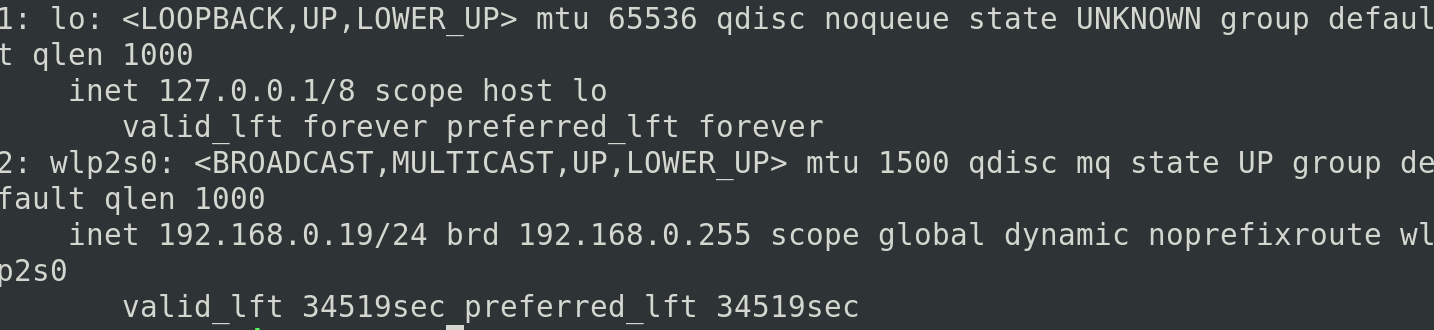
\includegraphics[width=10cm]{ressources/ip.png}
        \captionof{figure}{Adresse de la machine}
    \end{center}
    \begin{itemize}
        \item L'adresse du réseau est 192.168.0.0
        \item L'adresse de broadcast est 192.168.0.255
        \item On peut connecter 254 machines sur ce réseau
    \end{itemize}
    \note[item]{adresse 169.254... = quand machine n'obtient pas adresse via DHCP, elle s'en crée une}
\end{frame}
\section{Structure en étoile}
\begin{frame}
    \frametitle{Structure en étoile}

    \begin{center}
        \centering
        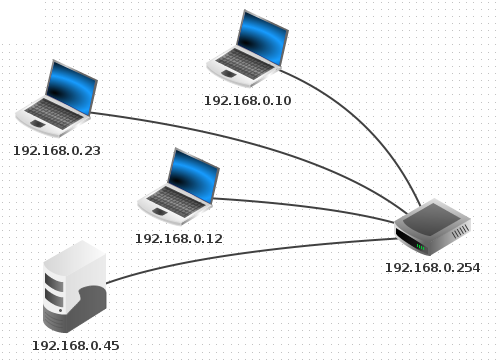
\includegraphics[width=8cm]{ressources/etoile.png}
        \captionof{figure}{\centering Les machines sont structurées en étoile autour du \textbf{routeur}.}
        \label{IMG}
    \end{center}

\end{frame}
\begin{frame}
    \frametitle{}

    \begin{aretenir}[]
        Un réseau est structuré autour d'un \textbf{routeur}.
        \begin{itemize}
            \item<1-> Il appartient au réseau. Il possède donc une adresse IP du réseau (par convention souvent la dernière disponible).
            \item<2-> Il route les informations d'un expéditeur vers le destinataire.
        \end{itemize}
    \end{aretenir}

\end{frame}
\section{Communiquer entre les réseaux}
\subsection{Passerelle}
\begin{frame}
    \frametitle{Communiquer entre les réseaux - passerelle}

    \begin{center}
        \centering
        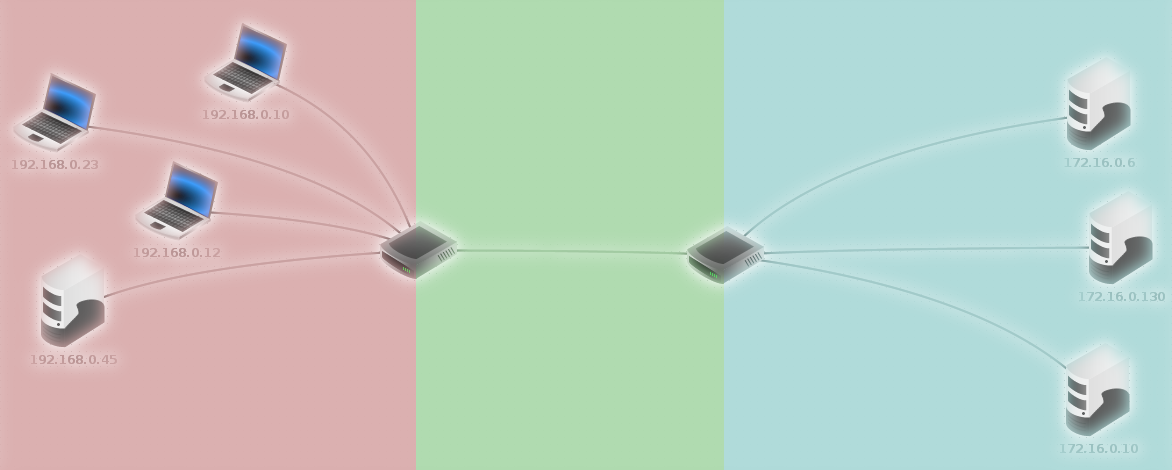
\includegraphics[width=10cm]{ressources/deuxreseaux.png}
        \captionof{figure}{Trois réseaux}
        \label{IMG}
    \end{center}

\end{frame}
\begin{frame}

    \begin{center}
        \centering
        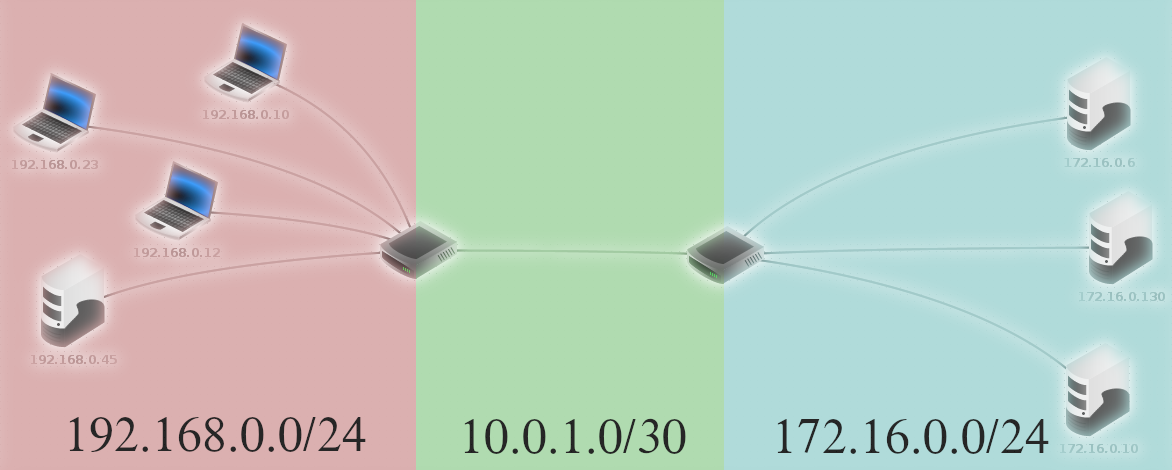
\includegraphics[width=10cm]{ressources/deuxreseaux2.png}
        \captionof{figure}{\centering Les routeurs appartiennent à deux réseaux.}
        \label{IMG}
    \end{center}

\end{frame}
\begin{frame}
    \frametitle{}

    \begin{aretenir}[]
        Un routeur est une passerelle entre plusieurs réseaux. Il possède autant d'\textbf{interfaces} que de réseaux associés.
    \end{aretenir}
    \begin{center}
        \centering
        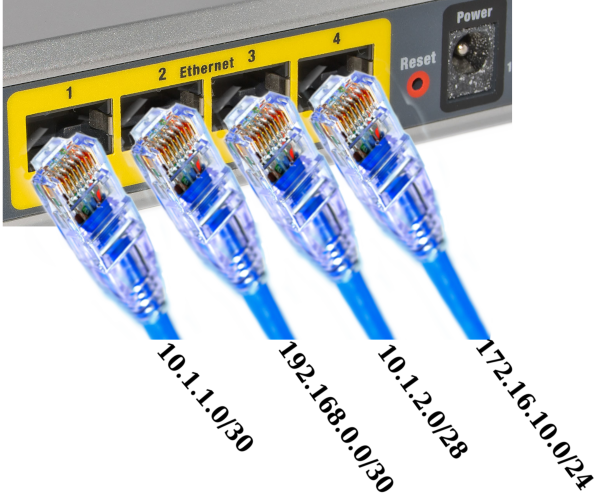
\includegraphics[width=5cm]{ressources/routeur-adresses.png}
        \captionof{figure}{Un routeur lié à quatre réseaux}
        \label{routeur}
    \end{center}
\end{frame}
\begin{frame}
    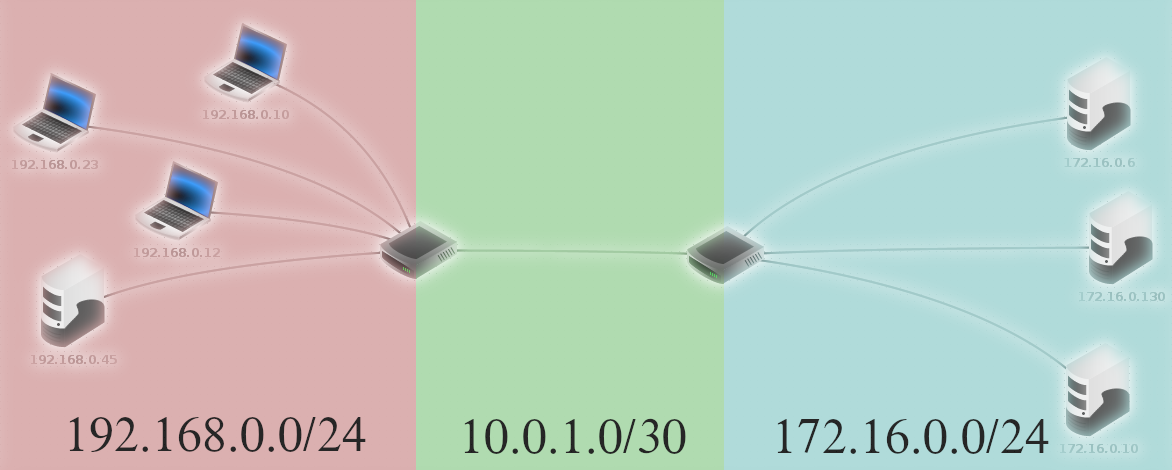
\includegraphics[width=10cm]{ressources/deuxreseaux2.png}
    Le routeur gauche possède deux interfaces; par exemple:
    \begin{itemize}
        \item 192.168.0.254
        \item 10.0.1.1
    \end{itemize}
    Le routeur droit possède deux interfaces; par exemple:
    \begin{itemize}
        \item 172.16.0.254
        \item 10.0.1.2
    \end{itemize}
\end{frame}
\subsection{Structure maillée}
\begin{frame}
    \frametitle{}
    Le réseau du lycée est partagé en plusieurs sous-réseaux.
    \begin{center}
        \centering
        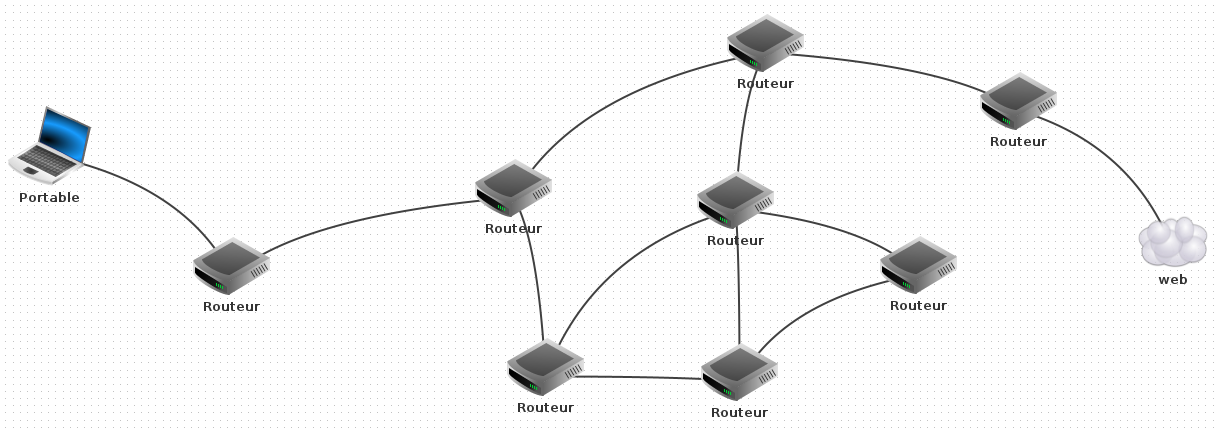
\includegraphics[width=10cm]{ressources/reseau.png}
        \captionof{figure}{Topologie d'un réseau}
        \label{reseau}
    \end{center}
    \note[item]{routeurs d'accès et internes}
\end{frame}
\begin{frame}
    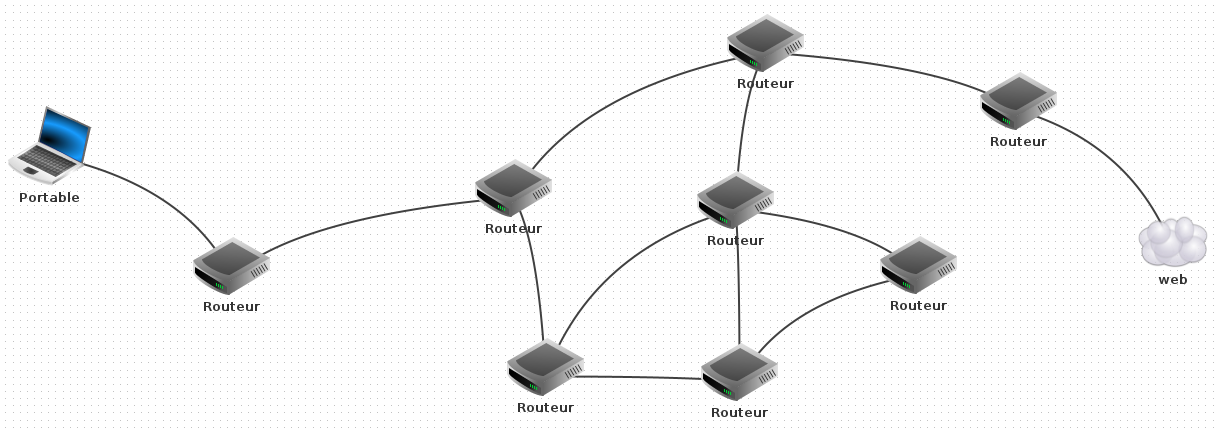
\includegraphics[width=10cm]{ressources/reseau.png}
    \begin{itemize}
        \item<1->Un paquet circule de \textbf{proche en proche}.
        \item<2-> Chaque routeur possède une \textbf{table de routage}.
        \item <3->La table de routage indique le prochain \emph{routeur voisin}.
        \item <4->La table de routage liste les routes d'accès à chaque réseau.
    \end{itemize}
    \note{Écritures différentes selon la littérature $\rightarrow$ on verra dans les exos}
\end{frame}


\begin{frame}[fragile]
    \begin{activite}
        Afficher la table de routage de la machine.
        \begin{lstlisting}[language=bash]
ip route
\end{lstlisting}
    \end{activite}
\end{frame}
\begin{frame}
    \frametitle{}

    \begin{center}
        \centering
        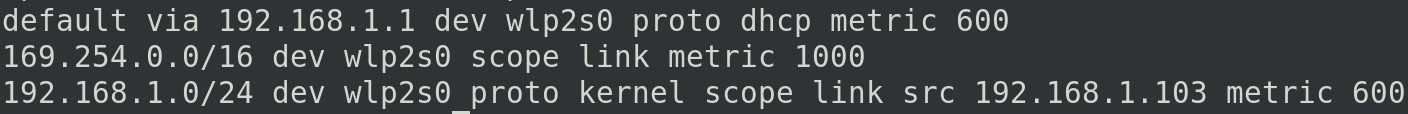
\includegraphics[width=10cm]{ressources/route.png}
        \captionof{figure}{Table de routage d'un ordinateur personnel}
        \label{IMG}
    \end{center}

\end{frame}

\begin{frame}[fragile]
    \frametitle{}
    \begin{activite}
        \begin{enumerate}
            \item Installer le paquet \texttt{\textbf{traceroute}}
                  \begin{center}
                      \begin{lstlisting}[language=bash, basicstyle=\ttfamily\small, xleftmargin=1em, xrightmargin=1em]
sudo apt install traceroute
\end{lstlisting}
                      \captionof{code}{Installation d'un paquet}
                      \label{ip}
                  \end{center}
            \item Taper la commande (code \ref{trace}).
                  \begin{center}
                      \begin{lstlisting}[language=bash, basicstyle=\ttfamily\small, xleftmargin=1em, xrightmargin=1em]
sudo traceroute -I fr.wikipedia.org
\end{lstlisting}
                      \captionof{code}{Tracer le chemin suivi vers une destination}
                      \label{trace}
                  \end{center}
        \end{enumerate}
    \end{activite}
\note[item]{Envoi de 3 paquets $\;\rightarrow\;$ donne une information moyenne}
\note[item]{La commande envoie des paquets avec un TTL (Time To Live) croissant pour découvrir la route au fur et à mesure.}
\note[item]{* * * ? La commande limite le TTL à 30; les serveurs rejettent les paquets UDP (User Datagram Protocol) (n'accepte que les TCP - Transmission Control Protocol)}
\note[item]{L'option -I de traceroute permet d'envoyer des paquets avec le protcole ICMP (Internet Control Message Protocol) = ping}
\end{frame}
\begin{frame}
    \frametitle{}
\begin{aretenir}[]
    Il n'y a pas de route définie entre l'émetteur et le destinataire. On parle de \textbf{commutation par paquets}.
\end{aretenir}
    \note[item]{Deux paquets qui partent de l'émetteur ne vont pas suivre le même chemin.}
    \note[item]{Commutation de circuits = liaison physique entre émetteur et destinaire $\;\rightarrow\;$ téléphone}
\end{frame}
\end{document}